\chapter{System Implementation}
\label{chap:implementation}

\section{Introduction}
\label{sec:impl_intro}
This chapter provides a detailed technical account of the implementation of the Smart Driving Behaviour Analysis System across all four operational tiers. It details the embedded firmware register configurations, the Bluetooth Low Energy (BLE) binary telemetry protocol, the cloud ingestion pipeline, the feature engineering and machine learning workflows, and the real-time web operations dashboard.

\section{Edge Sensor Firmware and BLE Telemetry Pipeline}
\label{sec:impl_edge}

\subsection{Embedded Hardware Register Configuration}
The edge node firmware is written in embedded C++ utilizing the Espressif IoT Development Framework. Direct two-wire I2C transactions operating at 400~kHz (Fast Mode) configure the internal control registers of the MPU-6050:
\begin{itemize}
    \item \textbf{Power Management 1 (\texttt{0x6B}):} Written with \texttt{0x01} to wake the sensor from sleep and select the internal Phase-Locked Loop (PLL) with the X-axis gyroscope reference as the clock source.
    \item \textbf{Accelerometer Configuration (\texttt{0x1C}):} Configured with byte \texttt{0x18}, setting bits \texttt{[4:3]} to \texttt{11}. This unlocks the full-scale acceleration range of $\pm 16g$ at a sensitivity of $2048\text{ LSB}/g$, ensuring unclipped collision impulse capture.
    \item \textbf{Gyroscope Configuration (\texttt{0x1B}):} Configured with byte \texttt{0x18}, setting bits \texttt{[4:3]} to \texttt{11}. This unlocks the full-scale angular rate range of $\pm 2000^\circ/\text{s}$ at a sensitivity of $16.4\text{ LSB}/(^\circ/\text{s})$.
    \item \textbf{Digital Low-Pass Filter (\texttt{0x1A}):} Configured with byte \texttt{0x03}, selecting a 44~Hz accelerometer filter bandwidth and 42~Hz gyroscope bandwidth. This hardware-level filtering suppresses high-frequency engine acoustic resonance and alternator electrical ripple.
\end{itemize}

\subsection{20-Byte Packed Binary Telemetry Frame}
To achieve high throughput and minimize radio transmission overhead, telemetry measurements are packed into a compact, contiguous 20-byte binary structure that fits within the standard 23-byte BLE Maximum Transmission Unit (MTU) without packet fragmentation. Table~\ref{tab:ble_packet} specifies the binary memory layout.

\begin{table}[H]
\centering
\small
\caption{20-Byte Binary BLE Telemetry Packet Specification}
\label{tab:ble_packet}
\begin{tabularx}{\textwidth}{llllX}
\toprule
\textbf{Byte Offset} & \textbf{Field} & \textbf{Data Type} & \textbf{Scale Factor} & \textbf{Description} \\
\midrule
$0 - 1$ & $a_x$ & \texttt{int16\_t} & $\times 100$ & Longitudinal G-force ($-16.00g \text{ to } +16.00g$) \\
$2 - 3$ & $a_y$ & \texttt{int16\_t} & $\times 100$ & Lateral G-force ($-16.00g \text{ to } +16.00g$) \\
$4 - 5$ & $a_z$ & \texttt{int16\_t} & $\times 100$ & Vertical G-force ($-16.00g \text{ to } +16.00g$) \\
$6 - 7$ & $\omega_x$ & \texttt{int16\_t} & $\times 10$ & Pitch angular rate ($-2000.0^\circ/\text{s} \text{ to } +2000.0^\circ/\text{s}$) \\
$8 - 9$ & $\omega_y$ & \texttt{int16\_t} & $\times 10$ & Roll angular rate ($-2000.0^\circ/\text{s} \text{ to } +2000.0^\circ/\text{s}$) \\
$10 - 11$ & $\omega_z$ & \texttt{int16\_t} & $\times 10$ & Yaw angular rate ($-2000.0^\circ/\text{s} \text{ to } +2000.0^\circ/\text{s}$) \\
$12 - 13$ & $\text{vib}$ & \texttt{int16\_t} & $\times 100$ & Dynamic vibration amplitude ($\text{m/s}^2$) \\
$14 - 17$ & $t$ & \texttt{uint32\_t} & $1$ & Microcontroller millisecond epoch timestamp \\
$18 - 19$ & $\text{CRC}$ & \texttt{uint16\_t} & $1$ & CRC16-CCITT packet verification checksum \\
\bottomrule
\end{tabularx}
\end{table}

\subsection{Mobile Client Gateway Implementation}
The mobile application is built in Flutter using the \texttt{flutter\_blue\_plus} library. The client scans for advertisements with the designated 128-bit Telematics Service UUID, establishes an authenticated connection, and enables notifications on the primary telemetry characteristic. 

Incoming binary payloads are unpacked, validated against the CRC16 checksum, and fused with the 1~Hz smartphone GPS coordinate stream. To preserve device battery and prevent GPU thermal throttling, the user interface updates are throttled using a reactive timer:
\begin{lstlisting}[language=Java, caption={Flutter UI Rebuild Throttling Mechanism}]
// Throttle sensor stream rebuilds to ~8.3 Hz (120ms)
_telemetrySubscription = BleService.stream.throttleTime(
  const Duration(milliseconds: 120),
  trailing: true,
).listen((packet) {
  _currentGForce = packet.acceleration;
  _currentYaw = packet.yawRate;
  notifyListeners();
});
\end{lstlisting}

\section{Cloud Telemetry Ingestion and Preprocessing Pipeline}
\label{sec:impl_cloud}
The cloud backend is deployed as an asynchronous FastAPI application running under Uvicorn with asynchronous PostgreSQL drivers. 

\subsection{Pydantic Schema Validation}
Incoming HTTP payloads are strictly validated at the API boundary using Pydantic schemas, enforcing boundary constraints on velocities ($0 \le v \le 200\text{ km/h}$) and valid latitude/longitude coordinates before database transactions occur.

\subsection{Spatial Downsampling Implementation}
To eliminate redundant database writes when vehicles are halted at red lights or in traffic congestion, the backend implements the 3-meter spatial delta filter:
\begin{lstlisting}[language=Python, caption={Python 3-Meter Spatial Downsampling Filter}]
def filter_stationary_breadcrumbs(points: list[TelemetryPoint]) -> list[TelemetryPoint]:
    if not points:
        return []
    filtered = [points[0]]
    for pt in points[1:]:
        last_pt = filtered[-1]
        d_lat = abs(pt.latitude - last_pt.latitude)
        d_lng = abs(pt.longitude - last_pt.longitude)
        # Threshold: ~0.000027 degrees corresponds to ~3.0 meters
        if d_lat >= 0.00003 or d_lng >= 0.00003:
            filtered.append(pt)
    return filtered
\end{lstlisting}

\section{Feature Extraction and Engineering}
\label{sec:impl_features}
High-frequency inertial time series collected from road trials are partitioned into sliding analysis windows of $W = 2.0\text{ seconds}$ with a step size of $\Delta W = 1.0\text{ second}$ (50\% temporal overlap), yielding 40 discrete samples per window at 20~Hz. 

For each temporal window, a 16-dimensional kinematic feature vector is computed across the signals $a_x(t)$, $a_y(t)$, $a_z(t)$, and ground speed $v(t)$:
\begin{enumerate}
    \item \textbf{Statistical Moments:} Arithmetic Mean ($\mu_x, \mu_y, \mu_z$) and Sample Standard Deviation ($\sigma_x, \sigma_y, \sigma_z$).
    \item \textbf{Kinematic Extremes:} Minimum and Maximum longitudinal acceleration ($\min(a_x), \max(a_x)$) and lateral acceleration ($\min(a_y), \max(a_y)$).
    \item \textbf{Peak-to-Peak Amplitude:} Long-range displacement $\Delta a_x = \max(a_x) - \min(a_x)$ and $\Delta a_y = \max(a_y) - \min(a_y)$.
    \item \textbf{Root Mean Square (RMS):} Total signal energy across the window:
    \begin{equation}
        \text{RMS}_a = \sqrt{\frac{1}{N} \sum_{k=1}^N \left(a_{x,k}^2 + a_{y,k}^2 + a_{z,k}^2\right)}
    \end{equation}
    \item \textbf{Maximum Jerk Derivative:} Maximum rate of acceleration change $\max\left|\frac{\Delta a}{\Delta t}\right|$.
    \item \textbf{Velocity Delta ($\Delta v$):} Speed differential over the window $\Delta v = v_{\text{end}} - v_{\text{start}}$.
\end{enumerate}

\section{Machine Learning Model Training and Classification}
\label{sec:impl_ml}
The classification framework aims to categorize temporal windows into four mutually exclusive operational maneuvers:
\begin{itemize}
    \item \textbf{Class 0 (Normal Cruising):} Stable velocity with smooth steering.
    \item \textbf{Class 1 (Harsh Braking):} Rapid negative longitudinal deceleration.
    \item \textbf{Class 2 (Rapid Acceleration):} Abrupt positive longitudinal acceleration.
    \item \textbf{Class 3 (Aggressive Swerving / Cornering):} High lateral centrifugal acceleration with simultaneous yawing.
\end{itemize}

\subsection{Supervised Classification Models}
The supervised learning pipeline was implemented using \texttt{scikit-learn}. The dataset was partitioned using stratified train-test splitting (80\% training, 20\% testing) to maintain class proportions. Continuous features were standardized using \texttt{StandardScaler} ($z = \frac{x - \mu}{\sigma}$).

Two primary classification models were trained and hyperparameter-tuned:
\begin{enumerate}
    \item \textbf{Random Forest Classifier:} An ensemble of $N=100$ decision trees, trained using Gini impurity with a maximum tree depth of 12 and minimum split samples of 4 to prevent overfitting to specific vehicle suspension characteristics.
    \item \textbf{Support Vector Machine (SVM):} Employing a non-linear Radial Basis Function (RBF) kernel with regularization parameter $C=10.0$ and kernel coefficient $\gamma = 0.1$, determined through 5-fold grid search cross-validation.
\end{enumerate}

\subsection{Unsupervised Driver Profiling via $k$-Means Clustering}
At the macroscopic trip level, an unsupervised $k$-Means model was fitted on normalized trip summary metrics (Harsh Braking rate per 100~km, Rapid Acceleration rate per 100~km, Swerving rate per 100~km, and Percentage of time spent overspeeding). Setting $k=3$ partitioned the driver cohort into three intuitive behavioral archetypes:
\begin{itemize}
    \item \textbf{Cluster 0 (Cautious):} Low event rates ($<1.5$ events/100~km) and minimal speed variance.
    \item \textbf{Cluster 1 (Normal / Moderate):} Moderate event rates (2.0 to 5.0 events/100~km) typical of urban stop-and-go driving.
    \item \textbf{Cluster 2 (Aggressive):} High event rates ($>8.0$ events/100~km) characterized by recurrent harsh braking and cornering.
\end{itemize}

\section{Web Command Dashboard and GIS Integration}
\label{sec:impl_dashboard}
The tactical operations dashboard is implemented in React 18, Vite, and TypeScript. Figure~\ref{fig:dashboard_preview} shows the interface architecture.

\begin{figure}[H]
    \centering
    % Placeholder for Dashboard Screenshot
    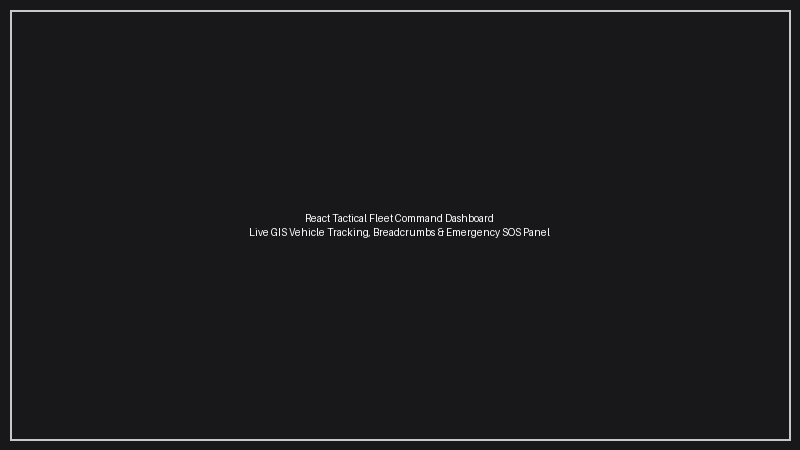
\includegraphics[width=0.88\textwidth]{figures/dashboard_preview.png}
    \caption{React Tactical Command Center with Live GIS Vehicle Tracking and Safety Metrics}
    \label{fig:dashboard_preview}
\end{figure}

The frontend integrates the following key modules:
\begin{itemize}
    \item \textbf{Interactive GIS Map Layer:} Rendered using \texttt{react-leaflet} and OpenStreetMap tiles. Vehicle positions are rendered as custom SVG markers dynamically rotated using CSS \texttt{transform: rotate($\theta$deg)} to mirror real-time vehicle compass headings.
    \item \textbf{Dynamic Breadcrumb Coloring:} Historical vehicle trajectories are rendered as SVG polyline segments dynamically color-coded based on instantaneous driver safety state: green for steady cruising, amber for minor road roughness or warnings, and red for harsh maneuvers or potholes.
    \item \textbf{Emergency SOS Dispatch Banner:} A WebSocket listener receives critical collision alerts ($\Delta V > 35\text{ km/h}$). Upon triggering, an audible alarm and a high-priority alert banner appear on the dispatcher's HUD, displaying the exact WGS-84 coordinates, driver contact details, and a one-click emergency dispatch button.
\end{itemize}
